\begin{table*}[t]
\centering
\caption{Main results (mean $\pm$ std over 3 seeds). Strict test excludes every test text seen in train or dev. Climate is direct transfer with no climate training. cw = class-weighted loss.}
\label{tab:main}
\setlength{\tabcolsep}{4pt}
\begin{tabular}{lrrcccc}
\toprule
Model & Params & Train (s) & Dev M-F1 & Strict Acc & Strict M-F1 & Climate M-F1 \\
\midrule
TF-IDF + LR & 101K & 2 & 0.489 $\pm$ 0.000 & 0.523 $\pm$ 0.000 & 0.473 $\pm$ 0.000 & 0.127 $\pm$ 0.000 \\
TF-IDF + LR (cw) & 101K & 1 & 0.498 $\pm$ 0.000 & 0.523 $\pm$ 0.000 & 0.475 $\pm$ 0.000 & 0.128 $\pm$ 0.000 \\
CNN & 437K & 13 & 0.444 $\pm$ 0.026 & 0.473 $\pm$ 0.016 & 0.423 $\pm$ 0.028 & 0.078 $\pm$ 0.012 \\
CNN (cw) & 437K & 8 & 0.449 $\pm$ 0.035 & 0.464 $\pm$ 0.007 & 0.426 $\pm$ 0.012 & 0.090 $\pm$ 0.034 \\
BiLSTM-Att & 584K & 10 & 0.391 $\pm$ 0.022 & 0.419 $\pm$ 0.014 & 0.358 $\pm$ 0.014 & 0.116 $\pm$ 0.007 \\
BiLSTM-Att (cw) & 584K & 9 & 0.357 $\pm$ 0.046 & 0.346 $\pm$ 0.086 & 0.333 $\pm$ 0.091 & 0.083 $\pm$ 0.028 \\
DistilBERT & 67.0M & 130 & 0.621 $\pm$ 0.010 & 0.585 $\pm$ 0.008 & 0.533 $\pm$ 0.008 & 0.133 $\pm$ 0.024 \\
DistilBERT (cw) & 67.0M & 123 & 0.632 $\pm$ 0.017 & 0.603 $\pm$ 0.005 & \textbf{0.554 $\pm$ 0.010} & 0.146 $\pm$ 0.013 \\
\bottomrule
\end{tabular}
\end{table*}


\subsection{Main comparison}
Table~\ref{tab:main} gives the full results. The two DistilBERT variants are the best models on every in-domain measure. The class-weighted variant has the highest dev macro-F1 (\devBertCw{}) and is therefore our selected model; on the strict test it reaches macro-F1 \fBertCw{}\,$\pm$\,\sdBertCw{} and accuracy \accBertCw{}, and the unweighted variant reaches \fBert{}\,$\pm$\,\sdBert{}. Selection uses the dev set only, so the choice does not rely on test data. The TF-IDF baseline is the best model without pretraining (\fTfidf{}), ahead of both neural models trained from scratch: the CNN reaches \fCnn{}\,$\pm$\,\sdCnn{} and the BiLSTM \fLstm{}\,$\pm$\,\sdLstm{}. A bag of n-grams therefore beats learned embeddings when only \nTrain{} training sentences are available, and the extra sequence modelling of the BiLSTM does not pay off at this scale. The non-pretrained models also vary more across seeds, which is expected given random embedding initialisation on a small corpus.

On the official test, which still contains the \nSeen{} previously seen sentences, every learned model scores higher than on the strict subset (DistilBERT-cw \offBertCw{}, CNN \offCnn{}). The two subsets differ in composition, so the gap is not a pure memorisation estimate, but it shows that reported LOGIC numbers depend on how overlap is handled.

Fig.~\ref{fig:comparison} places in-domain and transfer scores side by side. Training time grows from about a second for TF-IDF to roughly \timeBert{}\,s per DistilBERT run on a laptop GPU, which is still cheap enough for repeated seeds.

\begin{figure}[t]
\centering
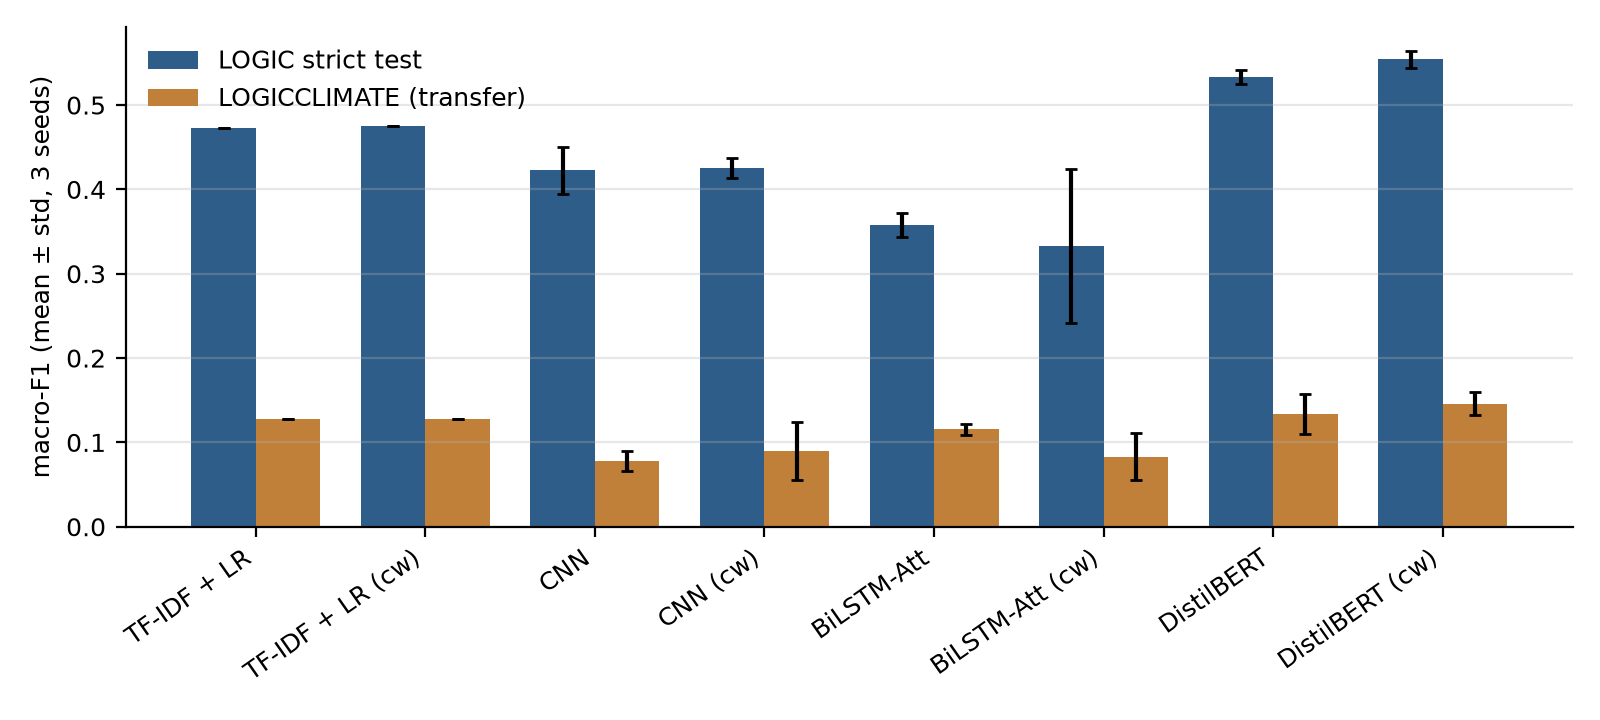
\includegraphics[width=\columnwidth]{../figures/final/model_comparison.png}
\caption{Strict-test and LOGICCLIMATE macro-F1 (mean $\pm$ std over \nSeeds{} seeds).}
\label{fig:comparison}
\end{figure}

\subsection{Is the difference real?}
Table~\ref{tab:sig} compares the selected model with every other configuration on the same strict-test rows. Against all TF-IDF, CNN and BiLSTM variants the paired bootstrap interval excludes zero and McNemar's test gives $p<0.01$, so the advantage of the pretrained encoder is not explained by test-set sampling. Against unweighted DistilBERT the difference is small and not significant under McNemar's test, so class weighting should be read as a minor refinement rather than a separate result.

\begin{table}[t]
\centering
\caption{Paired comparison of DistilBERT (cw) against each model on the strict test (seed 42): macro-F1 difference, 95\% paired-bootstrap interval (2{,}000 resamples) and exact McNemar $p$.}
\label{tab:sig}
\setlength{\tabcolsep}{4pt}
\begin{tabular}{lccc}
\toprule
Versus & $\Delta$M-F1 & 95\% CI & $p$ \\
\midrule
TF-IDF + LR & +0.087 & [+0.034, +0.146] & 0.002 \\
TF-IDF + LR (cw) & +0.085 & [+0.030, +0.141] & 0.004 \\
CNN & +0.143 & [+0.080, +0.205] & $<$0.001 \\
CNN (cw) & +0.124 & [+0.067, +0.182] & $<$0.001 \\
BiLSTM-Att & +0.201 & [+0.131, +0.270] & $<$0.001 \\
BiLSTM-Att (cw) & +0.163 & [+0.094, +0.227] & $<$0.001 \\
DistilBERT & +0.036 & [+0.002, +0.074] & 0.122 \\
\bottomrule
\end{tabular}
\end{table}


\subsection{Per-class behaviour and imbalance}
\begin{table}[t]
\centering
\caption{Per-class strict-test F1 (seed mean) for CNN and DistilBERT (cw), ordered by training frequency $n$.}
\label{tab:perclass}
\begin{tabular}{lrcc}
\toprule
Class & $n$ & CNN & DistilBERT (cw) \\
\midrule
faulty generalization & 314 & 0.52 & 0.64 \\
ad hominem & 219 & 0.56 & 0.74 \\
false causality & 167 & 0.43 & 0.65 \\
ad populum & 150 & 0.62 & 0.76 \\
circular reasoning & 131 & 0.58 & 0.55 \\
appeal to emotion & 127 & 0.37 & 0.50 \\
fallacy of logic & 119 & 0.32 & 0.39 \\
fallacy of relevance & 111 & 0.25 & 0.49 \\
intentional & 110 & 0.27 & 0.30 \\
false dilemma & 109 & 0.74 & 0.85 \\
fallacy of credibility & 107 & 0.18 & 0.47 \\
fallacy of extension & 100 & 0.57 & 0.60 \\
equivocation & 37 & 0.07 & 0.28 \\
\bottomrule
\end{tabular}
\end{table}

Table~\ref{tab:perclass} and Fig.~\ref{fig:perclass} break the scores down by class. Frequency is not the only factor. \emph{False dilemma}, a mid-frequency class with a distinctive surface form (``either \ldots\ or''), is the easiest class for the selected model, while \emph{equivocation}, the rarest class with 37 training sentences, remains the hardest for every model. The broad ``fallacy of'' categories (\emph{logic}, \emph{relevance}, \emph{credibility}) and \emph{intentional} are weak across the board. These labels are defined by what the argument does rather than by recognisable wording, and they overlap with more specific classes. The most frequent errors of the seed-42 DistilBERT model confirm this: \emph{faulty generalization} predicted as \emph{fallacy of logic}, and \emph{fallacy of relevance} predicted as \emph{fallacy of extension}.

Class weighting was expected to help rare classes. Its effect depends on the model (Fig.~\ref{fig:cw}): it gives DistilBERT a small gain spread over several classes, barely changes the CNN on average and hurts the BiLSTM, whose seed variance also grows. It never lifts \emph{equivocation} or \emph{intentional} above 0.30 F1. With fewer than 40 examples, reweighting the loss cannot supply the missing variety of phrasings.

\begin{figure*}[t]
\centering
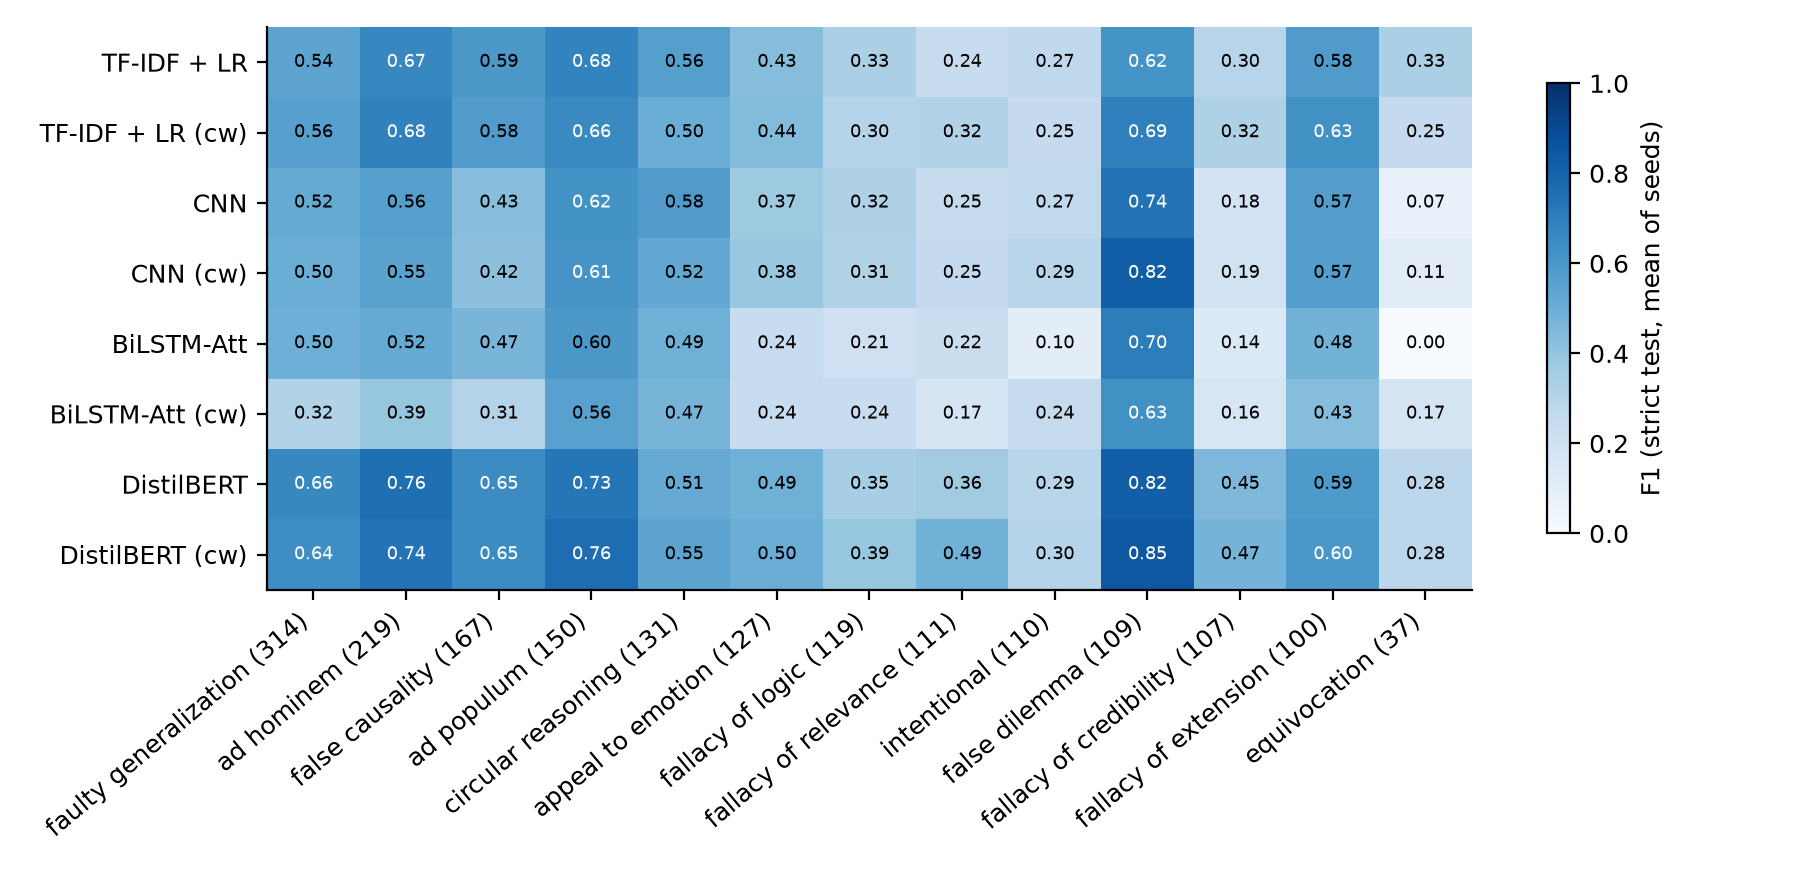
\includegraphics[width=0.85\textwidth]{../figures/final/per_class_f1.png}
\caption{Per-class strict-test F1 (seed mean). Columns are ordered by training frequency, shown in brackets.}
\label{fig:perclass}
\end{figure*}

\begin{figure}[t]
\centering
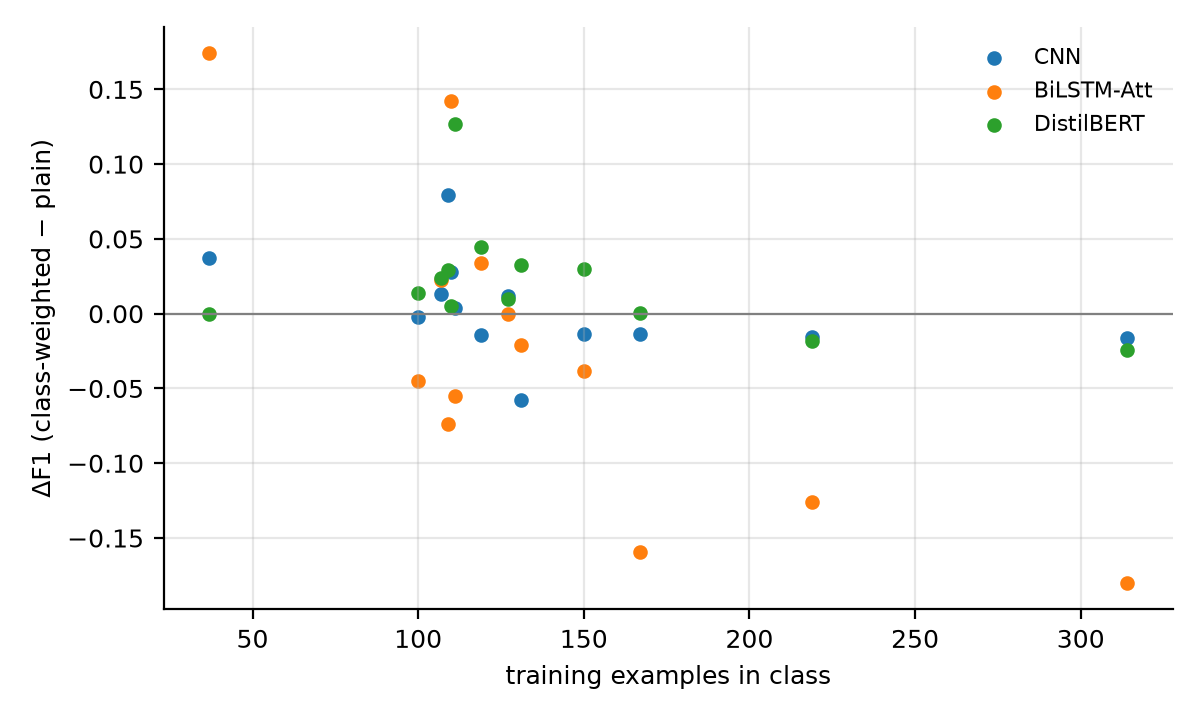
\includegraphics[width=0.92\columnwidth]{../figures/final/class_weighting_effect.png}
\caption{Change in per-class F1 from class weighting, plotted against class frequency.}
\label{fig:cw}
\end{figure}

\subsection{Transfer to climate news}
Applied without adaptation to LOGICCLIMATE, every model collapses (Table~\ref{tab:main}, last column). The best transfer macro-F1 is \climBertCw{} for class-weighted DistilBERT and \climTfidf{} for TF-IDF; the CNN falls to \climCnn{}. Climate sentences come from journalism rather than quizzes and follow a different label distribution in which \emph{intentional} is the most common class. Jin et al.\ reported a similar drop for their structure-aware model~\cite{jin2022logical}. In-domain gains therefore do not carry over to real discourse, and domain adaptation remains the main open problem for this line of work.

\subsection{Explanations}
For each prediction the interface removes one word at a time and records the drop in the predicted class's probability, a text version of occlusion analysis~\cite{zeiler2014visualizing}. We ran this probe over the correctly classified strict-test sentences of five classes with the seed-42 DistilBERT model and counted each sentence's two most influential words. For \emph{ad populum} the word \emph{everyone} was among them in 11 sentences; for \emph{false dilemma}, \emph{or} appeared 7 times and \emph{either} 3 times; for \emph{circular reasoning}, \emph{because} appeared 7 times. These are exactly the surface cues a human would point to. Such scores are useful for spotting shortcut cues, but they measure sensitivity rather than reasoning, and we do not use them as evidence that a model understands the argument.

\begin{figure}[t]
\centering
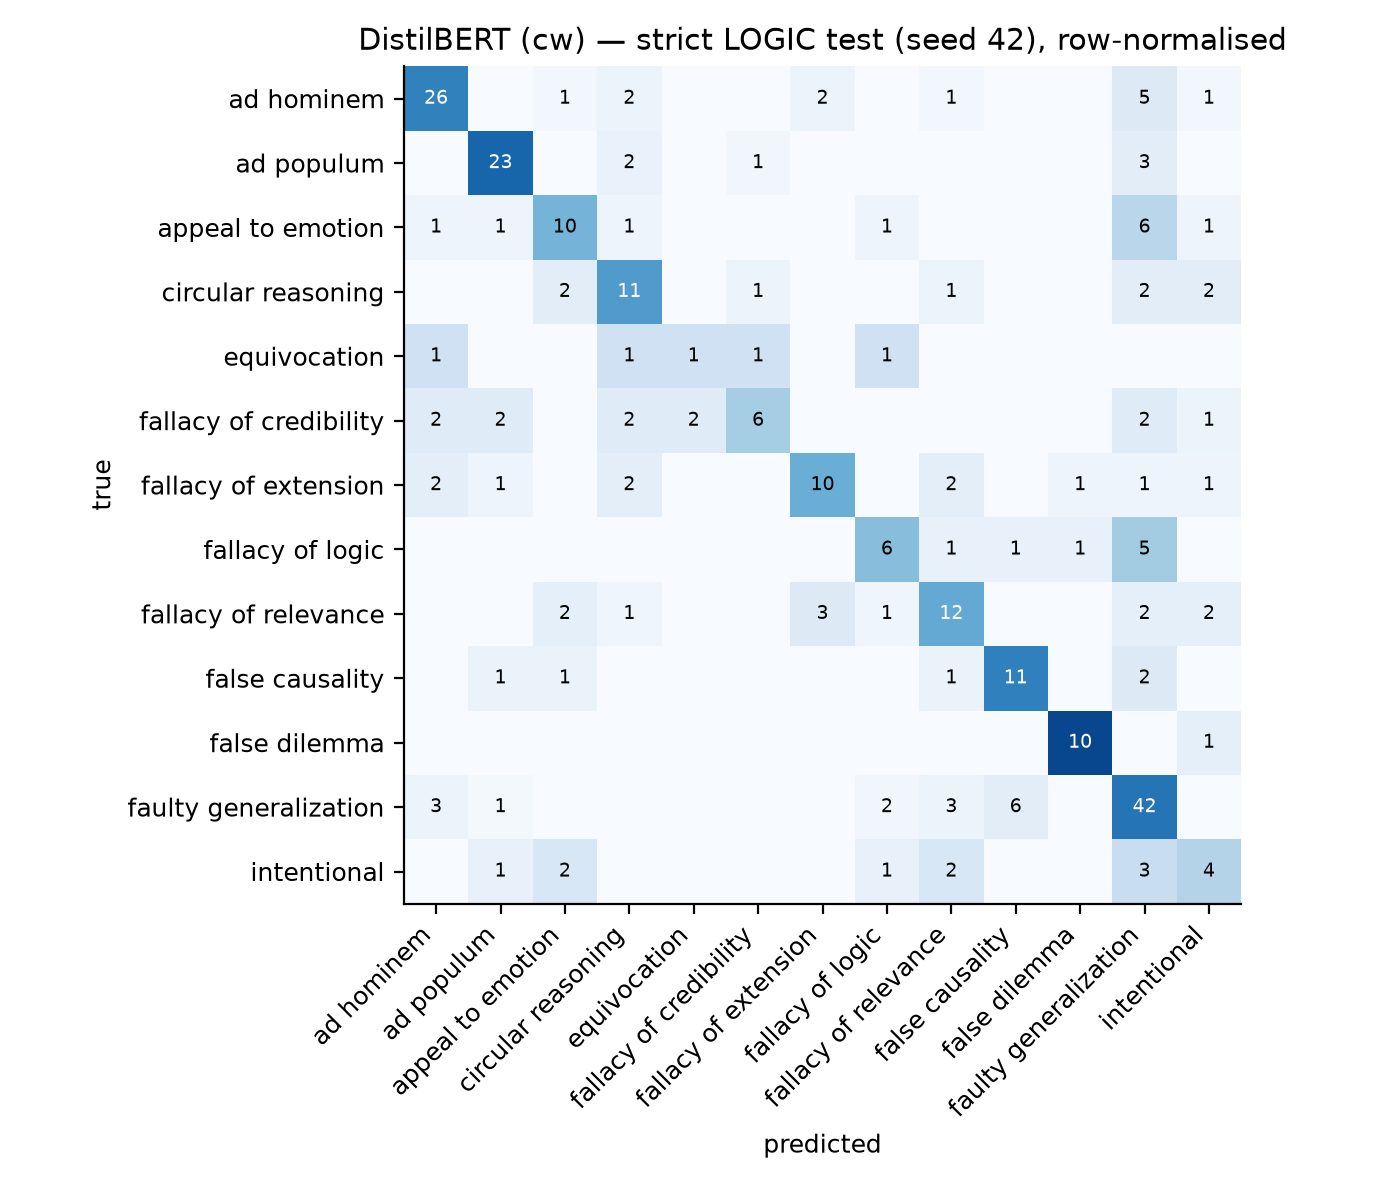
\includegraphics[width=0.95\columnwidth]{../figures/final/confusion_matrix_selected.png}
\caption{Row-normalised confusion matrix of the selected model (DistilBERT, class-weighted) on the strict test (seed 42); cells show counts.}
\label{fig:cm}
\end{figure}
